\documentclass[
]{beamer}

\usepackage[english]{babel}
%\usepackage[utf8]{inputenc}
\usepackage[T1]{fontenc}
\usepackage{booktabs}


\setbeamertemplate{frametitle}[default][left]
\setbeamercolor{page number in head/foot}{fg=black}
\setbeamerfont{page number in head/foot}{size=\small}

\setbeamertemplate{footline}[page number]

\begin{document}
	
	\title[]{Deep Survival Models for High-Dimension Data}
	%\subtitle[Short Presentation Subtitle]{Response Surface Methodology}
	\date{\today}
	\subject{Presentation Subject}
	
	\begin{frame}[plain]
		\maketitle
	\end{frame}
	
	
	\begin{frame}[plain]
		\begin{itemize}
			\item Predicting clinical outcomes from
			large scale cancer genomic profiles
			with deep survival models (SurvivalNet)
			\item A Deep Learning-Based Radiomics
			Model for Prediction of Survival in
			Glioblastoma Multiforme
		\end{itemize}
		
	\end{frame}
	
	\section{SurvivalNet}
	\begin{frame}[plain]{SurvivalNet}{Problems}
		\begin{itemize}
			\item Traditional Cox proportional hazards models require enormous cohorts for training models on
			high-dimensional datasets containing large numbers of features. 
			\item  A small set of features is
			selected in a subjective process that is prone to bias and limited by imperfect understanding of disease biology.
		\end{itemize}
	\end{frame}
	
	\begin{frame}[plain]{SurvivalNet}{Possible Model}
		\begin{itemize}
			\item  Cox proportional hazards models with  elastic net regularization.
			\item  Random survival forests.
			\item  Neural network based approaches(SurvivalNet)
		\end{itemize}
	\end{frame}
	
	\begin{frame}[plain]{SurvivalNet}{Cox proportional hazards models with  elastic net regularization}
		\begin{figure}
			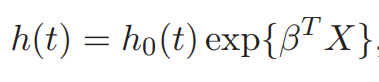
\includegraphics[scale=0.5]{cox1}\\
			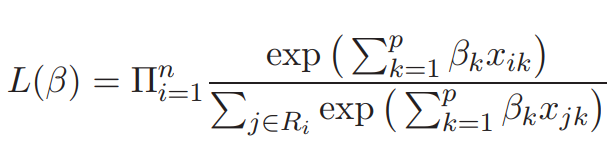
\includegraphics[scale=0.5]{cox2}\\
			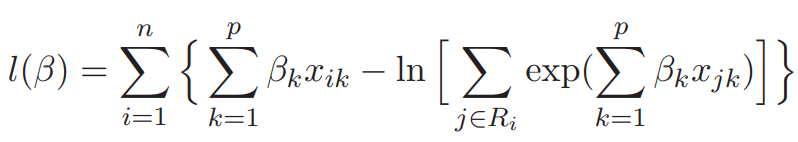
\includegraphics[scale=0.5]{cox3}\\
			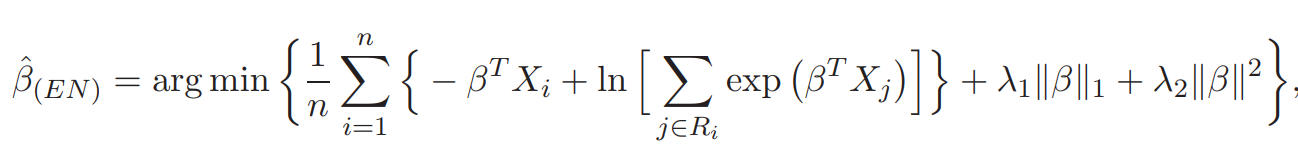
\includegraphics[scale=0.29]{cox4}
		\end{figure}
	\end{frame}
	
	\begin{frame}[plain]{SurvivalNet}{Random survival forests}
		\begin{figure}
			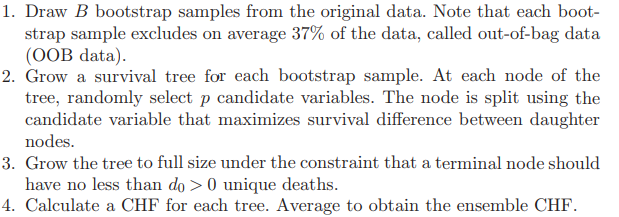
\includegraphics[scale=0.6]{rsf}
		\end{figure}
	\end{frame}
	
	\begin{frame}[plain]{SurvivalNet}{Overview}
		\begin{figure}
			\centering
			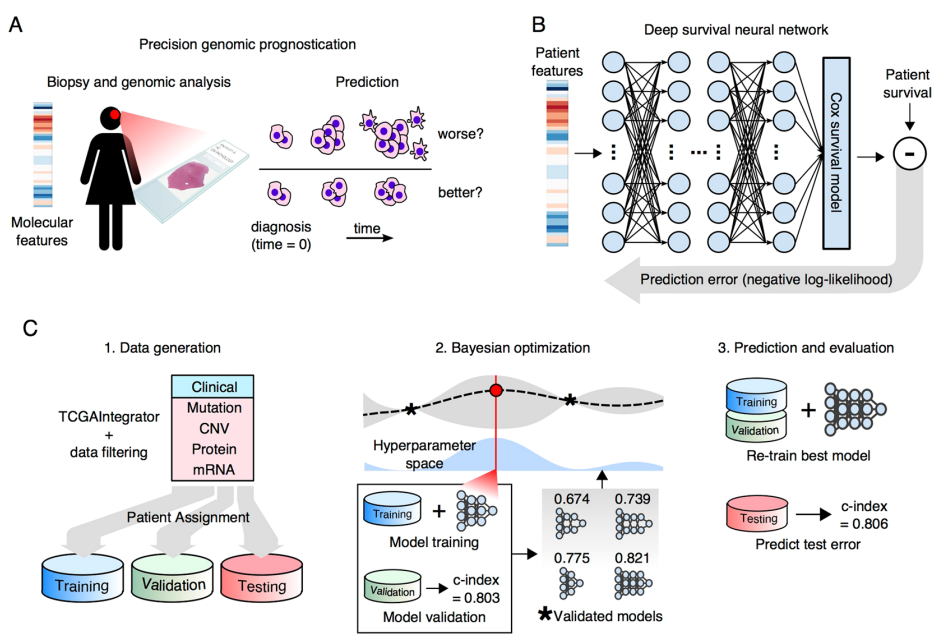
\includegraphics[scale=0.45]{snover}
		\end{figure}
	\end{frame}
	
	
	\begin{frame}[plain]{Data Splitting}
		\begin{figure}
			\centering
			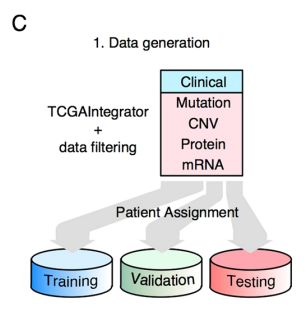
\includegraphics[scale=0.4]{split}
		\end{figure}
		\begin{itemize}
			\item All datasets were created and filtered using TCGAIntegrator.
			\item Data is first split into training (60\%), validation (20\%), and
			testing (20\%) sets
			\item Performance was evaluated
			with two feature-sets: 1) a "transcription" feature set containing 17,000 + gene expression features obtained
			by RNA-sequencing, and 2) an "integrated" feature set containing 3-400 features describing clinical features,
			mutations, gene and chromosome arm-level copy number variations, and protein expression features.
		\end{itemize}
	\end{frame}
	
	
	\begin{frame}[plain]{Deep survival neural network}
		\begin{figure}
			\centering
			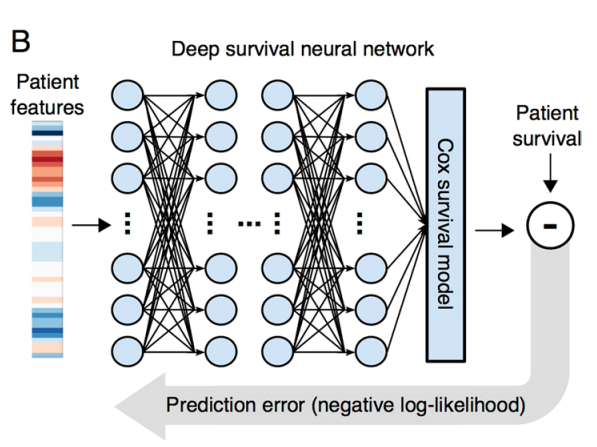
\includegraphics[scale=0.4]{nn1}
		\end{figure}
		\begin{itemize}
			\item Fully connected hidden layer is used. 
			\item input is the feature, output is log-likelihood of Cox proportional hazards model.
		\end{itemize}
	\end{frame}
	
	\begin{frame}[plain]{Deep survival neural network}
		\begin{figure}
			\centering
			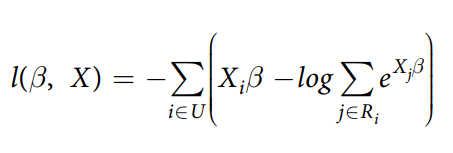
\includegraphics[scale=0.5]{loglik1}
		\end{figure}
		\begin{itemize}
			\item $X_i$ are the inputs to output layer
			\item $\beta$ are the Cox model parameters
			\item $U$ is the set of events
			\item $R_i$ is the set of "at risk" samples.
		\end{itemize}
		\begin{figure}
			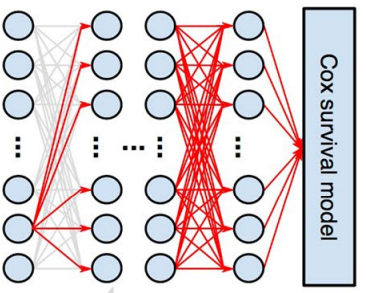
\includegraphics[scale=0.5]{nn2}
		\end{figure}
	\end{frame}
	
	\begin{frame}[plain]{Bayesian optimization for hyper-parameter tuning}
		\begin{figure}
			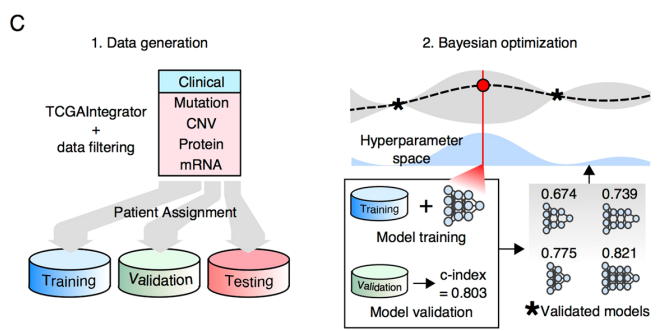
\includegraphics[scale=0.3]{bayes1}
		\end{figure}
		\begin{itemize}
			\item Hyper-parameters of the deep learning structure includes number of layers, number
			of elements in each layer,  number and type of activation functions in each layer,  choices for optimization/regularization procedures,  dropout fraction...
			\item Bayesian optimization enables users
			who lack experience tuning neural networks to optimize model designs automatically, and results in considerable
			savings in time and effort as previously reported.
		\end{itemize}
	\end{frame}
	
	\begin{frame}{Bayesian optimization for hyper-parameter tuning}
		\begin{itemize}
			\item Training samples are used to train the model weights with backpropagation using the network
			design suggested by Bayesian optimization.
			\item The prediction accuracy of the trained deep survival model is then
			estimated using the validation samples, and is used to maintain a probabilistic model of performance as a function
			of hyperparameters.
			\item  Based on the probabilistic model, the design with the best expected accuracy is inferred
			as the next design to test.
		\end{itemize}
	\end{frame}
	
	
	\begin{frame}{Model comparison results}
		\begin{figure}
			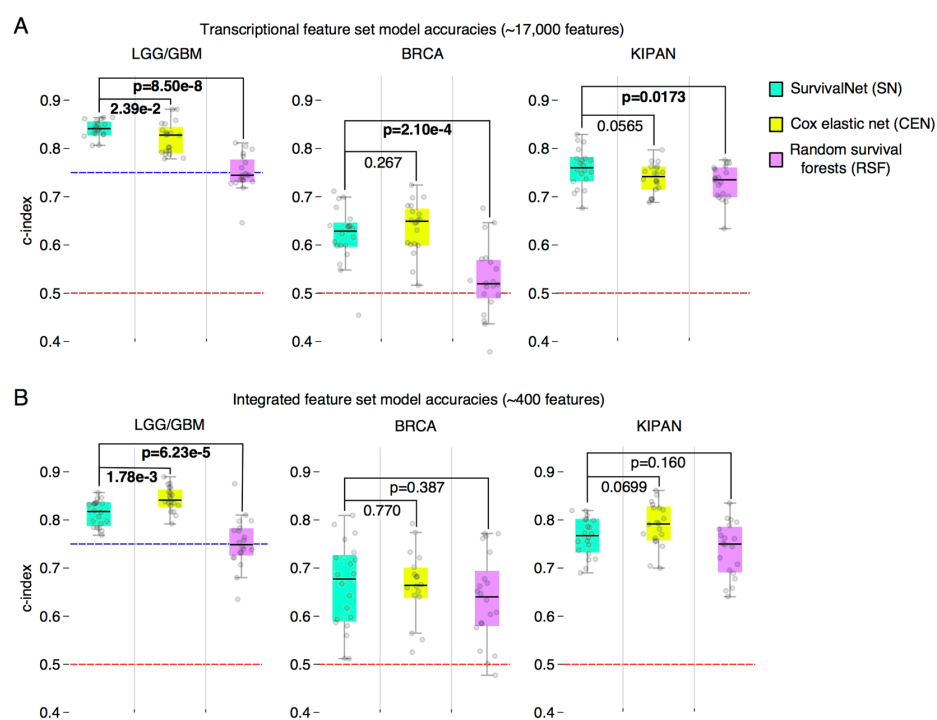
\includegraphics[scale=0.4]{res1}
		\end{figure}
	\end{frame}
	
	\begin{frame}
		\begin{itemize}
			\item Both SN and CEN significantly outperform RSF models in most experiments.
			\item Performance is generally better on the integrated feature set than the transcriptional feature set for all methods.
			\item RSF models have the
			worst performance generally.
			\item Comparing performance across diseases,
			we noticed that prediction accuracy generally decreases as the proportion of right-censored samples in a dataset
			increases. This pattern holds for all prediction methods. Glioma had the highest overall prediction accuracy,
			being a uniformly fatal disease that has relatively fewer long-term survivors and incomplete follow-up (62-64\%).
			Breast carcinoma had the lowest overall prediction accuracy with more than 86-91\% of BRCA samples being
			right-censored.
		\end{itemize}
	\end{frame}
	
	\begin{frame}{Interpreting deep survival models with risk backpropagation}{Linear survival model}
		\begin{itemize}
			\item Linear survival models weight individual
			features based on their contribution to overall risk, providing a clear interpretation of the prognostic significance
			of individual features, and insights into the biology of disease progression.
		\end{itemize}
		\begin{figure}
			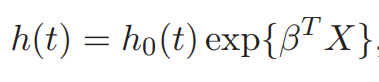
\includegraphics[scale=0.5]{cox1}
		\end{figure}
	\end{frame}
	
	\begin{frame}{Interpreting deep survival models with risk backpropagation}{Risk backpropagation}
		\begin{itemize}
			\item  The prediction can be conceptualized instead as a nonlinear surface where the risk gradients change
			depending on a patient's feature values, and so these feature weights are calculated separately for each patient.
			\item The models used for risk backpropagation and
			interpretation were created by identifying the best performing model configuration from the randomized
			experiments.
		\end{itemize}
		\begin{align*}
		\frac{\partial R}{\partial f}=\beta\times\prod_{h=1}^{H} J_h
		\end{align*}
		\begin{itemize}
			\item $H$ number of hidden layers, $R$ risk, $J_h$ Jacobian matrix of the $h$-th hidden layer with respect to its inputs, $\beta$ is the vector of parameters
			of the final layer that is a linear transformation
		\end{itemize}
	\end{frame}
	
	
	\begin{frame}
		\begin{figure}
			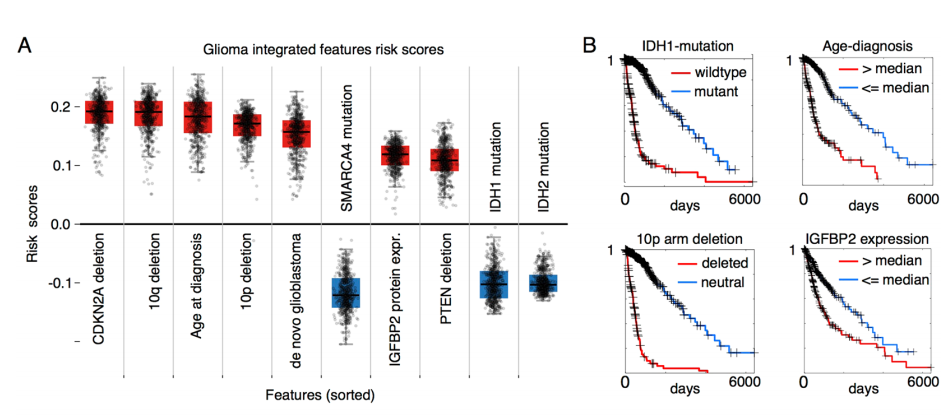
\includegraphics[scale=0.4]{fea1}
		\end{figure}
	\end{frame}
	
	
	\begin{frame}{Transfer learning with multi-cancer datasets}
		\begin{itemize}
			\item Perform a series of transfer learning experiments
			to evaluate the ability of deep survival models to benefit from training with data from multiple cancer
			types
			\item  Survival models were trained using three different
			datasets: BRCA-only, BRCA+OV (ovarian serous carcinoma), and BRCA+OV+UCEC (corpus endometrial
			carcinoma), and were evaluated for their accuracy in predicting BRCA outcomes
			\item The large proportion of
			right-censored cases in the BRCA dataset (90\%) makes training accurate models difficult, and so we hypothesized
			that augmenting BRCA training data with samples from other hormone-driven cancers could improve BRCA
			prognostication 
			\item Datasets were combined using their shared features. 
			
		\end{itemize}
	\end{frame}
	
	\begin{frame}
		\begin{figure}
			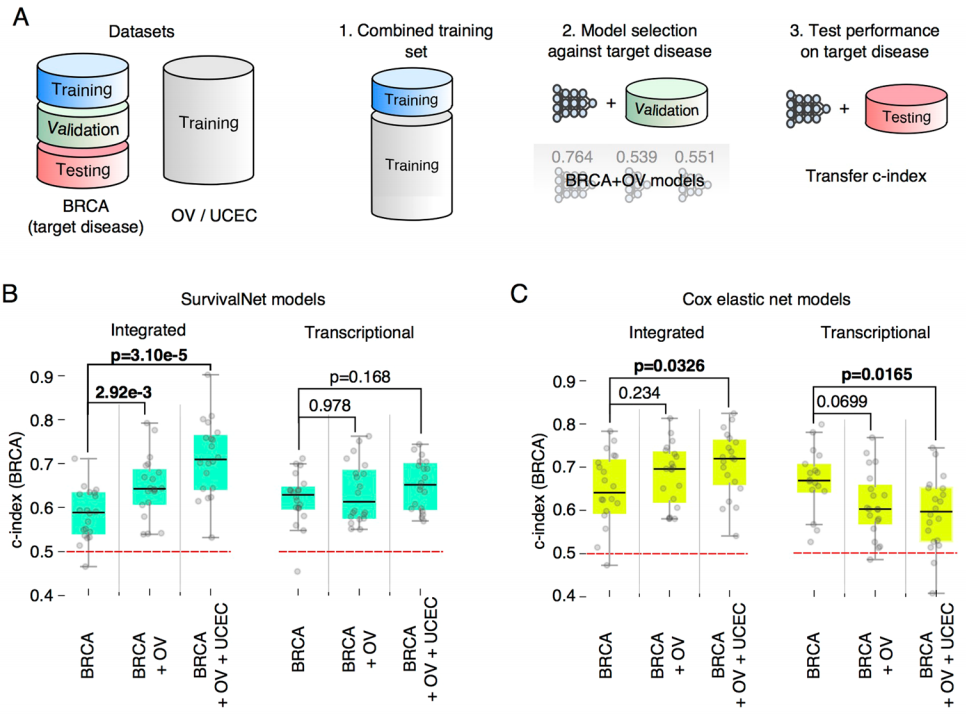
\includegraphics[scale=0.45]{trans1}
		\end{figure}
	\end{frame}
	
	\begin{frame}{Discussion}
		We created a software framework for Bayesian optimization and interpretation of deep survival models, and evaluated
		the ability of optimized models to learn from high-dimensional and multi-cancer datasets. Our software
		enables investigators to efficiently construct deep survival models for their own applications without the need for
		expensive manual tuning of design hyperparameters, a process that is time consuming and that requires considerable
		technical expertise. We also provide methods for model interpretation, using the backpropagation of risk to
		assess the prognostic significance of features and to gain insights into disease biology. Our analysis shows the ability
		of deep learning to extract important prognostic features from high-dimensional genomic data, and to effectively
		leverage multi-cancer datasets to improve prognostication. It also reveals limitations in deep learning for
		survival analysis and the value of complex and deeply layered survival models that need to be further investigated.
	\end{frame}
	
	%%%another paper
	\begin{frame}{A Deep Learning-Based Radiomics
			Model for Prediction of Survival in
			Glioblastoma Multiforme}{Overview}
		\begin{figure}
			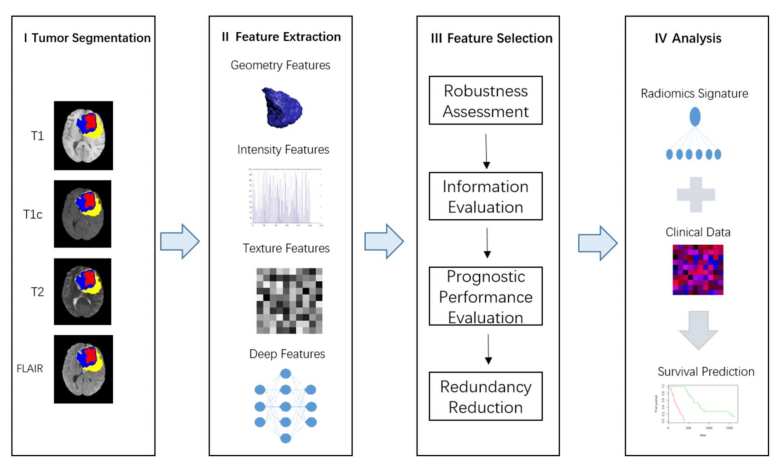
\includegraphics[scale=0.5]{over2}
		\end{figure}
	\end{frame}
	
	\begin{frame}{Datasets}
		\begin{itemize}
			\item  A total of 112 patients (62 men and 50 women; mean age, 54.640 years $\pm$44.040;
			range 10-84 years) with pathologically confirmed GBM were included.
			\item  The patient cohorts consisted of two
			groups: a discovery cohort comprising 75 patients from the Cancer Genome Archive (TCGA) database, and
			an independent validation cohort comprising 37 patients
			\item The inclusion criteria were that patients with newly diagnosed and treatment-naive GBM and
			survival information and pre-treatment MR imaging including T1-weighted, T1-weighted Gadolinium contrast-enhanced,
			T2-weighted, and T2-weighted FLAIR images (short for T1, T1C, T2, and FLAIR). The exclusion
			criteria are patients with a history of surgery or chemoradiation therapy and patients missing survival information.
		\end{itemize}
	\end{frame}
	
	\begin{frame}{Datasets}
		\begin{figure}
			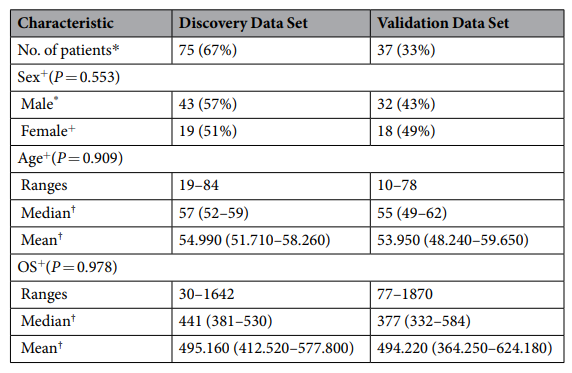
\includegraphics[scale=0.5]{data2}
		\end{figure}
	\end{frame}
	
	\begin{frame}{Image Preprocessing and Tumor Segmentation}
		\begin{itemize}
			\item  Images were re-sampled to 1mm$\times$1mm$\times$1mm
			\item Three tumor subregions were segmented, including the necrosis area, the enhancement area and the
			edema area.  The necrosis area was the low intensity necrotic structures within the enhancing rim in T1C and had
			hyper-intense signal in T2 and FLAIR. The enhancement area was confirmed as the Gadolinium enhancing rim
			excluding the necrotic center and hemorrhage with both T1C and T1 images. The edema area was identified as
			abnormality visible in T2 and FLAIR excluding ventricles and cerebrospinal fuid. The edema area may include
			both peritumoral edema and any non-enhancing tumor.
		\end{itemize}
	\end{frame}
	
	\begin{frame}{Feature Extraction}{Handcrafed Features}
		\begin{itemize}
			\item The handcrafed features were extracted from five subregions
			and four MR modalities. The feature extraction subregions include necrosis, enhancement, edema, tumor core
			(the whole tumor except edema) and whole tumor (necrosis, enhancement and edema). 
			\item The handcrafed features
			can be divided into three groups: (I) geometry, (II) intensity and (III) texture. 
			\item A total of
			1403 handcrafed features are extracted, including 23 geometry features, 340 intensity features, and 1040 texture
			features. 
		\end{itemize}
	\end{frame}
	
	\begin{frame}{Feature Extraction}{Deep Features}
		\begin{itemize}
			\item Deep features were extracted from pre-trained CNN via transfer learning. In this study, CNN\_S
			was chosen as the pre-trained CNN model.
			\item For each patient, the necrosis, tumor core and whole tumor subregions were chosen
			as input of CNN\_S.
		\end{itemize}
	\end{frame}
	
	\begin{frame}{Feature Extraction}{Deep Features}
		First, from multiple transverse slices in the segmentation volume, we picked out the slice
		which had the largest tumor area. Then, the gray values were normalized to range 
		$\left[0, 255\right]$ using linear transformation.
		Based on the segmentation results, the three tumor subregions were cropped from the selected slices
		in all four MR modalities. Next, each cropped subregion image was resized to 224$\times$224 with bicubic interpolation.
		The obtained images can be used as the model input. The G and B channels of CNN\_S were turned of
		so only grayscale images were allowed to enter the model. Finally, the deep features can be computed by only
		forward propagation and were extracted from fully-connected layer 6 and fully-connected layer 7.  In total, 98304 deep features can be extracted for each patients.(all weights of CNN\_S were predetermined)
	\end{frame}
	
	\begin{frame}{Feature Extraction}{Deep Features}
		\begin{figure}
			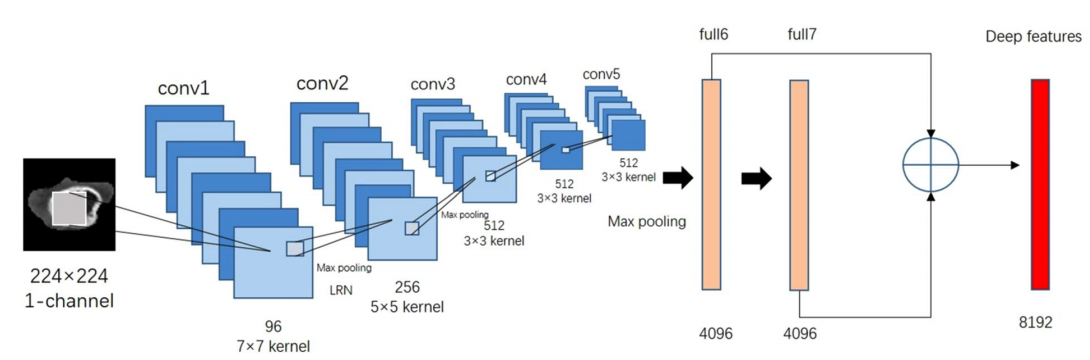
\includegraphics[scale=0.4]{cnn1}
		\end{figure}
	\end{frame}
	
	
	\begin{frame}{Feature Selection}
		\begin{itemize}
			\item After features extraction, all 1403 handcrafed features and 98304 deep features for each
			patients were normalized as z-scores. A four-step method is used for feature selection. All calculations are performed on the
			discovery data set.
			\item Test-retest analysis and inter-rater analysis were used to determine the feature robustness. Based on 30 patients
			randomly chosen from the discovery data set, the test-retest analysis was performed where for each patient the
			tumor subregions were segmented twice by one rater.
			\item The data set used for inter-rater analysis included
			another 30 randomly chosen patients, where for each patient the tumor subregions were segmented by two raters
			independently. The features extracted from these multiple-segmented subregions were assessed using intraclass
			correlation coefficient 
			\item  Feature with ICC$\leq0.85$ were considered as robust against intra- and inter-rater
			uncertainties.
		\end{itemize}
	\end{frame}
	
	\begin{frame}{Feature Selection}
		\begin{itemize}
			\item Then, the median absolute deviations (MAD) was calculated for each remained feature. Features with MAD
			equal to zero were discarded.
			\item Next, we further selected features with prognostic value. Here the prognostic performance is assessed
			using the concordance index (C-index).  Features with C-index$\geq$0.580 are considered.  After prognostic performance analysis, 1581 features remained
			as predictive factors.
			\item Then, we further reduced
			the data dimension by removing highly correlated features. Here the correlation coefficient between each pair of
			features is calculated. For feature pair with correlated coefficient ≥0.90, the more prognostic feature is retained
			and the other feature is removed. Finally, the remained 150 image features are selected and regarded as robust,
			predictive and non-redundant.
		\end{itemize}
	\end{frame}
	
	\begin{frame}{Statistical Analysis}{Signature Construction}
		\begin{itemize}
			\item Based on the selected 150 features, we aimed to construct a radiomics signature using
			multivariate Cox regression model for prediction of survival in GBM patients. Because there were more image
			features than patients, strong feature selection and shrinkage were still required to prevent overprinting as well as
			increase interpretation. To address this problem, the least absolute shrinkage and selection operator (LASSO) Cox
			regression model was used on the discovery data set for signature construction.
			\item  The retained features with nonzero coefficients were
			used for regression model fitting and combined into a radiomics signature. Subsequently, we obtained a radiomics
			score for each patient by a linear combination of retained features weighed by their model coefficients
		\end{itemize}
	\end{frame}
	
	\begin{frame}{Statistical Analysis}{Signature Validation}
		\begin{itemize}
			\item The association of the constructed signature with survival was assessed on the discovery
			data set and validated on the validation data set by using Kaplan-Meier survival analysis. Based on a threshold
			calculated using the radiomics score, all patients were stratified into high-risk and low-risk groups. The threshold
			was estimated based on the discovery data set by using an optimal cutpoint analysis with X-tile software, and
			tested on the validation data set. A weighted log-rank test (G-rho rank test, rho=1) was used to test the significant
			difference between the high-risk and low-risk groups. The C-Index was used to assess the performance of
			the signature.
		\end{itemize}
	\end{frame}
	
	\begin{frame}{Statistical Analysis}{Signature Validation}
		\begin{figure}
			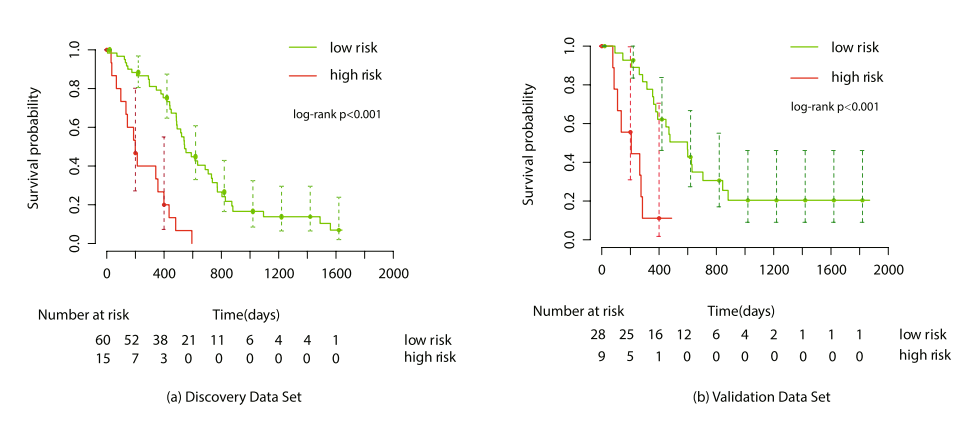
\includegraphics[scale=0.45]{km1}
			\caption{Illustration of Kaplan-Meier survival curve. The Kaplan-Meier survival curve show OS risk
				stratification for patients in Discovery data set (a) and Validation data set (b). Patients were classified as low risk
				and high risk according to radimics signature. The vertical dashed line is 95\% confdence interval.}
		\end{figure}
	\end{frame}
	
	\begin{frame}{Statistical Analysis}{Signature Validation}
		\begin{itemize}
			\item To assess the univariate predictive performance of each feature with non-zero LASSO coefficient, the univariate
			analysis was performed based on both discovery and validation data sets. To assess the univariate association
			with risk, each non-zero feature was used for patient stratification into high-risk and low-risk groups.
			\item To compare the built radiomics signature with other clinical risk factors such as age and KPS, the C-indices of
			these clinical risk factors were calculated based on both discovery and validation data sets. To assess the combination
			prognostic value of the signature with clinical factors, we put the radiomics signature together with clinical
			parameters into the Cox regression model. The model was fitted based on the discovery data set and validated on
			the validation data set. 
		\end{itemize}
	\end{frame}
	
	
	\begin{frame}{Results}{Clinical Characteristics and OS}
		The median and mean of OS were 441 days and 495.160 days for the discovery
		set, 377 days and 494.220 days for the validation set. The median and mean of age were 57 years and 54.990
		years for the discovery set, 55 years and 53.950 years for the validation set. The discovery set had 43 males and 32
		females, while the validation set had 19 males and 18 females. There was no significant difference in clinical and
		follow-up data between the discovery and validation data sets (P=0.553 for sex test, 0.748 for KPS test, 0.909 for
		age test, 0.302 for tumor volume test and 0.978 for OS test).
	\end{frame}
	
	
	
	\begin{frame}{Results}{Signature Construction}
		\begin{figure}
			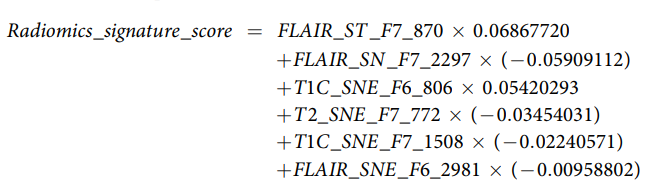
\includegraphics[scale=0.5]{form2}
		\end{figure}
	\end{frame}
	
	\begin{frame}
		\begin{figure}
			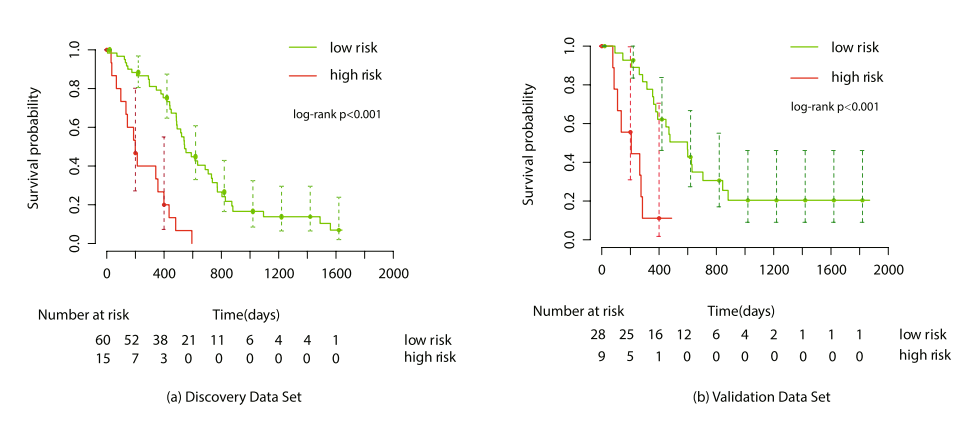
\includegraphics[scale=0.45]{km1}
			\caption{Illustration of Kaplan-Meier survival curve. The Kaplan-Meier survival curve show OS risk
				stratification for patients in Discovery data set (a) and Validation data set (b). Patients were classified as low risk
				and high risk according to radiomics signature. The vertical dashed line is 95\% confidence interval.}
		\end{figure}
	\end{frame}
	
	
\end{document}
